\textbf{Lý thuyết dây cho tương tác mạnh}

Theo Vật Lý hiện đại, thế giới tự nhiên được xây dựng dựa trên bốn lực tương tác cơ bản. Trong chương trình Vật Lý THPT, cũng như qua cuộc sống thường ngày, có lẽ các bạn đã không còn xa lạ với lực hấp dẫn và lực điện từ. Tuy nhiên, để giải thích các hiện tượng ở mức nguyên tử và nhỏ hơn, các nhà khoa học cần sử dụng thêm hai loại lực tương tác nữa: lực tương tác yếu và lực tương tác mạnh. Lý thuyết mô tả lực tương tác mạnh là {\it sắc động lực học lượng tử}, và theo lý thuyết này thì các hạt nhân nguyên tử -- hạt proton và hạt neutron -- có cấu tạo từ ba hạt quark, liên kết với nhau chủ yếu qua trường gluon. Các hạt được cấu tạo từ nhiều quark liên kết kiểu này có tên gọi chung là hadron. 

\begin{enumerate}
    \item \textbf{Quỹ đạo Regge của họ các hạt meson}\\
    Meson là các hạt hadron có cấu tạo từ hai quark. Xét một họ các hạt meson có liên hệ giữa khối lượng bình phương $M^2$ và spin $S$ (giá trị momen động lượng nội tại, tính theo đơn vị hằng số Planck rút gọn $\hbar$) như hình \ref{fig01}. Liên hệ này gần như tuyến tính $S = \alpha_0 + \alpha M^2$, là đặc trưng của tính chất quỹ đạo Regge, được quan sát trên rất nhiều họ các hạt meson khác nhau.

\begin{figure*}[!htbp]
\centering
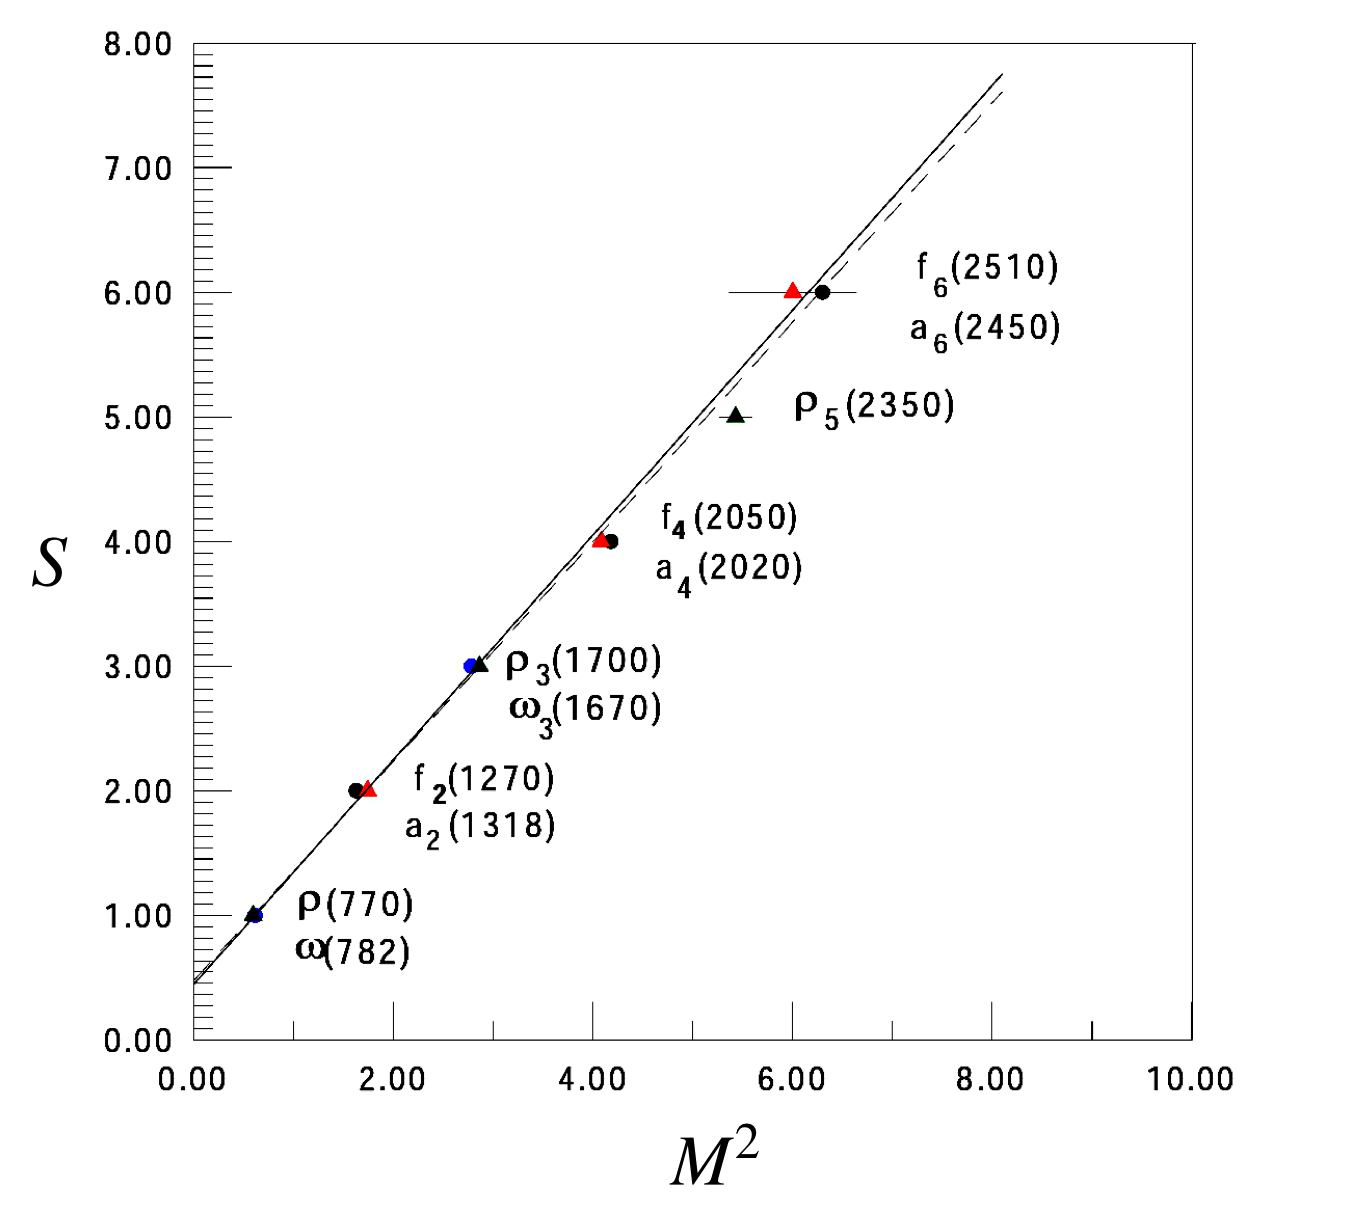
\includegraphics[width=0.6\textwidth]{Problem_20/fig01.png}%
\caption{Đồ thị Chew-Frautschi cho liên hệ gần như tuyến tính giữa khối lượng bình phương $M^2$ và spin (giá trị momen động lượng nội tại) $S$ của một họ các hạt meson.} %\cite{refId0}}
\label{fig01}
\end{figure*}
    
    Cho biết $M^2$ được tính theo đơn vị $($GeV$/c^2)^2$ với $c$ là giá trị vận tốc ánh sáng và $1$GeV $=1.60\times 10^{-10}$J. Hãy xác định hệ số tỉ lệ $\alpha$ của họ các meson trong hình \ref{fig01}. 
    
    \item \textbf{Mô hình dây tương đối tính của meson}\\
    Thành phần $\alpha M^2$ trong biểu thức của $S$ có thể được giải thích thông qua một mô hình dây quay tròn tương đối tính, như mô tả ở hình \ref{fig02}. Cụ thể, trong mô hình này, hai quark được nối với nhau bằng một ống dòng trường gluon tạo thành một dây có hai đầu nặng. Giả sử rằng các quark là những chất điểm có khối lượng nghỉ rất nhỏ $m \rightarrow 0$, và ống dòng trường gluon có mật độ năng lượng nghỉ $\lambda$ trên đơn vị chiều dài. Xét trạng thái chuyển động của hai quark là ở trên cùng một đường tròn, đứng yên trong hệ quy chiếu quan sát.

    \begin{figure*}[!htbp]
\centering
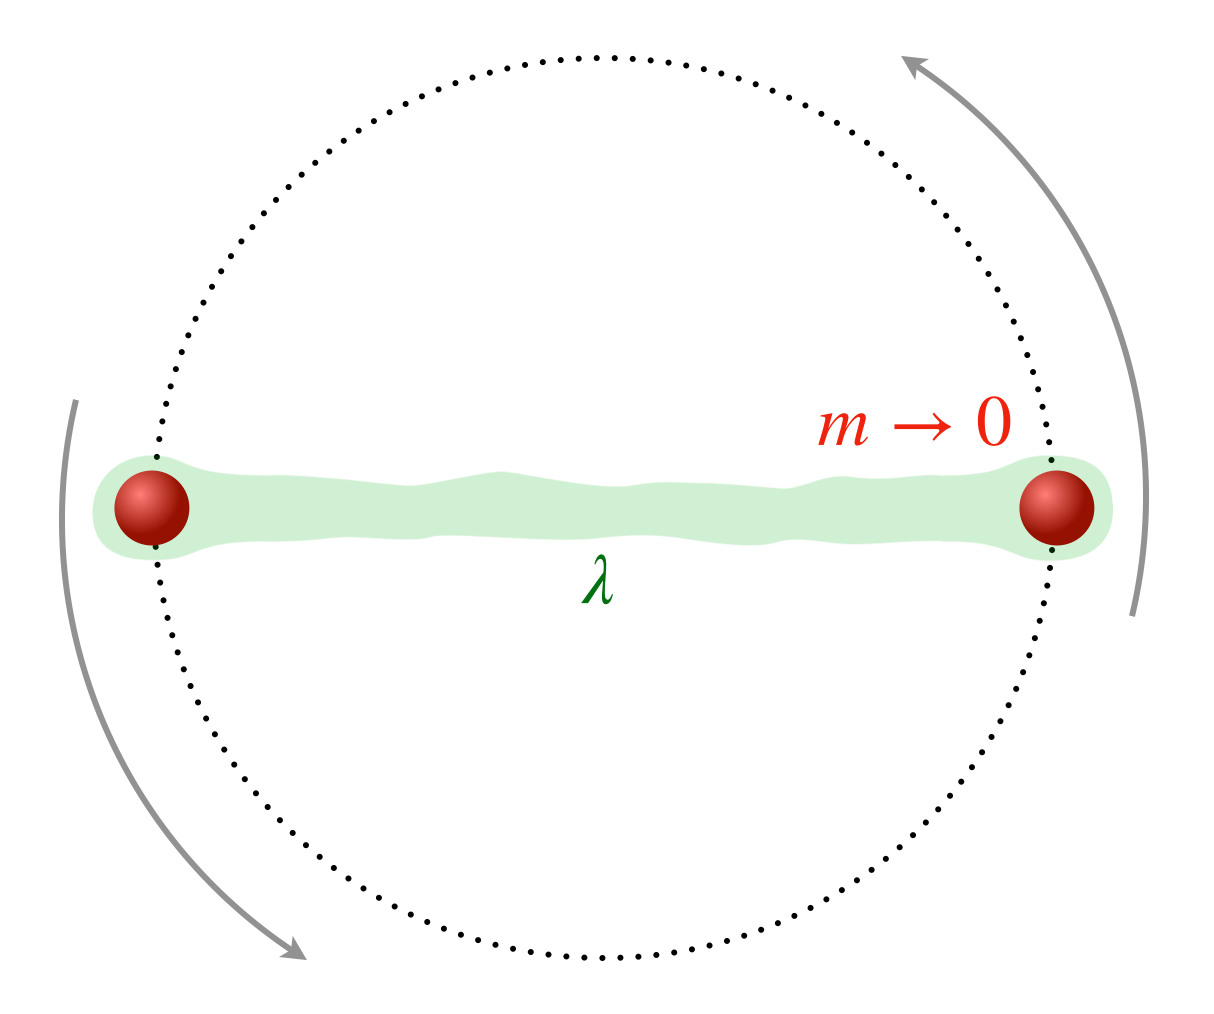
\includegraphics[width=0.6\textwidth]{Problem_20/fig02.png}%
\caption{Mô hình dây quay tròn tương đối tính của hạt meson, với giả sử rằng hai quark có khối lượng nghỉ $m\rightarrow 0$ và chuyển động trên cùng một đường tròn. Dây dự trữ mật độ năng lượng nghỉ $\lambda$ trên đơn vị chiều dài.}
\label{fig02}
\end{figure*}

    a/ Nếu momen động lượng của dây quay quanh tâm đường tròn là $J$, hãy xác định năng lượng $E$ của dây (cùng hai quark) trong hệ quy chiếu quan sát theo momen động lượng $J$ và mật độ năng lượng nghỉ $\lambda$. Bạn cần phải chứng minh rằng sự phụ thuộc của kết quả này vào khối lượng nghỉ $m$ các quark sẽ biến mất khi $m \rightarrow 0$.

    b/ Chúng ta liên hệ khối lượng $M$ của hạt meson với năng lượng $E$ của dây theo công thức tương đương năng - khối lượng Einstein $E=Mc^2$, và spin $S$ của meson với momen động lượng $J/\hbar$ của dây (tính theo đơn vị hằng số Planck rút gọn). Hãy xác định mật độ năng lượng nghỉ $\lambda$ theo giá trị $\alpha$ đã tìm được từ ý 1 của bài tập này.

    c/ Hãy xác định chiều dài $L$ của dây theo momen động lượng $J$ và hệ số $\alpha$. 
    
    \item \textbf{Nhiệt độ Hagedorn}\\
    Tương tác mạnh, như tên gọi của nó, là vô cùng mạnh -- ta gần như không thể quan sát được một hạt quark đơn lẻ ở trạng thái tự do, là đặc trưng cho tính chất giam cầm. Tuy nhiên, ở một giá trị nhiệt độ $T_{H}$ đủ lớn, được gọi là nhiệt độ Hagedorn, thì tương tác mạnh sẽ mất đi tính chất giam cầm và các quark sẽ được giải phóng, trở nên tự do -- hệ {\it sắc động lực học lượng tử} khi ấy sẽ ở trạng thái quark-gluon plasma.

    Ở các ý tiếp theo, chúng ta không những sẽ phải giải quyết một câu hỏi toán thống kê cụ thể, mà còn sẽ phải hiểu ý nghĩa Vật Lý của kết quả. Các bạn sẽ được cung cấp rất nhiều kiến thức mới, và yêu cầu phải sử dụng được chúng để giải quyết những câu hỏi.

    a/ Thay vì chỉ quay vòng quanh như mô hình tương đối tính trong hình \ref{fig02}, dây lượng tử có năng lượng và momen động lượng phụ thuộc vào trạng thái dao động của nó. Các giá trị momen động lượng khả dĩ của dây lượng tử (tính theo đơn vị hằng số Planck rút gọn) là tập hợp số nguyên không âm $J/\hbar =0,1,2,...$, và số lượng $\mathcal{N}[J/\hbar]$ các trạng thái dao động độc lập khác nhau cho mỗi giá trị momen động lượng $J/\hbar>0$ là bằng với số lượng các cách viết $J$ theo tổng của các số nguyên dương ($\mathcal{N}[0]=1$, tương ứng với trạng thái nền duy nhất). Các số hạng trong biẻu diễn tổng có thể lặp lại, nhưng các hoán đổi vị trí khác nhau chỉ được tính là một cách viết. Đây chỉ là một trong rất nhiều các liên hệ kỳ thú và sảng khoái giữa lý thuyết dây và lý thuyết số học.

    Chúng ta minh họa với $J/\hbar=4$. Có $5$ cách khác nhau để biểu diễn số $4$ theo tổng các số nguyên dương, là $1+1+1+1$, $1+1+2$, $1+3$, $2+2$, và $4$, cho nên $\mathcal{N}[4]=5$. Chú ý rằng, các trạng thái dao động khả dĩ của dây có thể xảy ra theo các phương khác nhau trong không gian, nhưng phép đếm $\mathcal{N}[J/\hbar]$ trên của chúng ta không hề đả động tới. Đây là một đơn giản hóa của bài tập. 

    Hãy xác định giá trị $\mathcal{N}[5]$, $\mathcal{N}[6]$, và $\mathcal{N}[7]$.

    b/ Hãy thành lập biểu thức ước tính chiều dài dây trung bình $\langle L \rangle$ ở nhiệt độ $T$, theo hàm $\mathcal{N}[J/\hbar]$, hệ số $\alpha$, hằng số Boltzmann $k_B$ và giá trị nhiệt độ $T$. Sử dụng kết quả đã tìm được ở ý 2a cho năng lượng $E$ dây quay tròn tương đối tính để ước tính năng lượng dây lượng tử, và 2c cho chiều dài $L$ dây quay tròn tương đối tính để ước tính chiều dài dây lượng tử, theo momen động lượng $J$ và hệ số $\alpha$. Giả sử rằng khi hệ {\it sắc động học lượng tử} ở nhiệt độ $T$ cân bằng thống kê thì xác suất dây sở hữu mỗi trạng thái mang năng lượng $E$ sẽ tuân theo phân bố Maxwell-Boltzmann -- tỉ lệ với $\exp(-E/k_B T)$.  

    c/ Chúng ta có thể xấp xỉ hàm $\mathcal{N}[J/\hbar]$ theo công thức Hardy-Ramanujan:
    \begin{equation}
        \mathcal{N}[J/\hbar] \approx \frac1{4\sqrt{3}(J/\hbar)} \exp \left[ \pi \sqrt{\frac{2(J/\hbar)}{3}} \right] \ ,
    \end{equation}
    áp dụng tốt nhất khi $J/\hbar \gg 1$. %\cite{LondonMathematical}
    
    Với kết quả tìm được ở ý 3b, vận dụng suy luận Vật Lý, hãy ước tính xem ở giá trị nhiệt độ bằng bao nhiêu thì các quark sẽ được giải phóng khỏi tính chất giam cầm. So sánh giá trị tìm được với nhiệt độ Hagedorn $T_H \sim 1.7 \times 10^{12}$K suy ra từ giả lập và thực nghiệm. %\cite{hadrons}
    
\end{enumerate}
    

\begin{flushright}
    (Biên soạn bởi XOONG)
\end{flushright}